\chapter{Resultados y Discusiones}
El siguiente capitulo se trabajo a base de la forma de validación detallada en el capitulo anterior. Esta incluye una reunión con un docente que imparte la materia de Fundamentos de Programación I y una prueba con estudiantes de una clase de esta materia. La reunión y experimentos se realizaron para ver la utilidad del producto realizado para usuarios finales potenciales.

\section{Detalles de resultados}
\subsection{Reunión con docente}
Se realizó una reunión el 6 de Octubre del 2021 con uno de los docentes del departamento de ingeniería eléctrica y computación de la UACJ que imparte la materia de Fundamentos de Programación I. En esta reunión, reviso el material del juego, se vio el valor didáctico de los diferentes puzzles del juego, y de manera menos detallada, la facilidad de montar el juego para el docente y el \textit{gameplay}. En la revisión del juego, comento de manera positiva la variedad de los puzzles. Sin embargo, comento que debido al diseño de los puzzles que algunos tienen código similar a \textit{C} (figura~\ref{fig:for_puzzle_fail_c}), otro muy parecido a \textit{Python} (figura~\ref{fig:for_puzzle_fail_python}) y algunos adicionales de pseudocódigo, seria complicado para el docente usar este juego para la impartición de su clase porque \textquotedblleft rompería \textquotedblright con lo visto en clase en algunos temas. Si el profesor tiene que explicar al estudiante que ciertos \textit{puzzles} funcionan de manera diferente a como se explico en clase, el juego pierda valor didáctico y en el peor de los casos, podría confundir a los estudiantes.
\begin{figure}
    \centering
    \begin{subfigure}{0.4\textwidth}
         \centering
         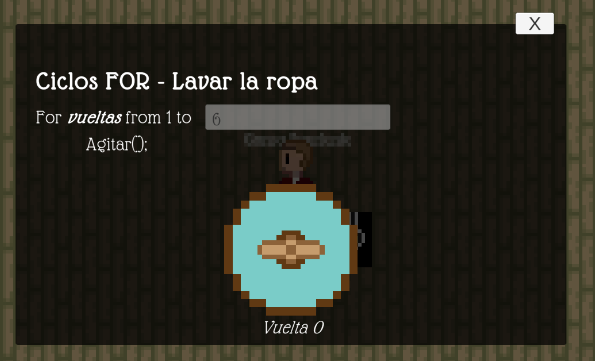
\includegraphics[width=\textwidth]{for_puzzle_fail_python}
         \caption{Este \textit{puzzle} tiene usa una sintaxis inspirada en \textit{Python} y su uso de \textit{ranges}}
         \label{fig:for_puzzle_fail_python}
     \end{subfigure}
         \begin{subfigure}{0.4\textwidth}
         \centering
         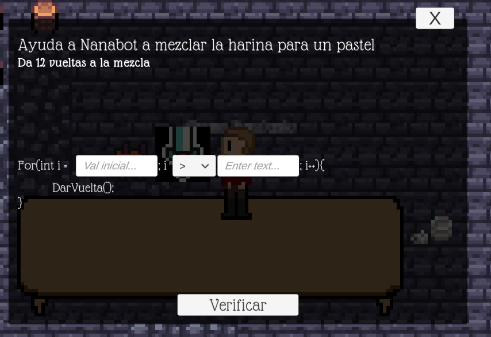
\includegraphics[width=\textwidth]{for_puzzle_fail_c}
         \caption{La sintaxis de este \textit{puzzle} es similar a C}
         \label{fig:for_puzzle_fail_c}
     \end{subfigure}
\end{figure}

Después de la reunión detallada anteriormente se arreglaron las cosas que evitaron que fuera verificado el producto para su uso en el salón de clases. Se decidió estandarizar todos los ejercicios para que usaran la sintaxis de PSeInt.

\subsection{Revisión con estudiantes}
Se definió que el día {dia} la realización de una prueba con la clase de Fundamentos de Programación 1 en el horario [horario]. De los x estudiantes de la clase, x número participaron en la prueba. Se inicio la prueba pidiendo a los alumnos que en el navegador web de su computadora personal entraran la url detallada anteriormente para que pudieran iniciar la prueba. Se pidió que contestaran una encuesta antes de iniciar el juego. Al iniciar el juego, [detallar cosas subjetivas que se notaron]. El juego tuvo una duración de [duración] minutos. Al terminar el juego se pidió que contestaran una encuesta dividida en dos partes:
\begin{itemize}
    \item Parte donde se pide a los estudiantes contestar ejercicios de los temas vistos en el juego, para medir si ocurre alguna mejora en el rendimiento después de jugar el juego.
    \item Otra sección donde se pide al alumno que evalué a base de una escala de 1 al 10 la diversión, usabilidad, ayuda didáctica del juego.
\end{itemize}